\documentclass[10pt,xcolor={dvipsnames}]{beamer}
\usepackage{polyglossia}
\usepackage{mathtools, amsthm, amssymb, amsfonts}
\usepackage{graphicx}
\setdefaultlanguage{french}
\usepackage{listings}
\usepackage{lstautogobble}

\usefonttheme{professionalfonts}
\usepackage{unicode-math}

\setmathfont{Latin Modern Math}
%\setmathfont[range={it}]{Latin Modern Sans 10 Oblique}
\setmathfont[range=up]{Latin Modern Sans}
\setmathfont[range={\mathbb}]{xits-math.otf}
%\setmathfont{xits-math.otf}
\setmonofont[Mapping=tex-text,Scale=0.9]{Consolas}

\lstset{language=Python,
	escapechar=\%,
	basicstyle=\ttfamily,
	keywordstyle=\color{OliveGreen}\ttfamily,
	stringstyle=\color{red}\ttfamily,
	commentstyle=\color{brown}\ttfamily,
	morecomment=[l][\color{blue}]{\#},
	columns=fixed,
	tabsize=4,
	autogobble=true
	keepspaces=false
}

%\usetheme{Frankfurt}
\usetheme{Hannover}
\usecolortheme{dolphin}

\newcommand{\N}{\mathbb N}
\newcommand{\Z}{\mathbb Z}
\newcommand{\R}{\mathbb R}
\newcommand{\Q}{\mathbb Q}
\newcommand{\CC}{\mathbb C}
\newcommand{\K}{\mathbb K}
\DeclarePairedDelimiter{\intcc}{[\![}{]\!]}

\newcounter{Exercice}
\resetcounteronoverlays{Exercice}
\makeatletter
\newenvironment{exo}[1][\@nil]{
	\def\tmp{#1}
	\refstepcounter{Exercice}
	\begin{block}{\textbf{Exercice \theExercice}
			\ifx\tmp\@nnil
			%
			\else
			(#1)
			\fi
		}
	}{\end{block}}
\makeatother

\newcounter{Exemple}
\resetcounteronoverlays{Exemple}
\makeatletter
\newenvironment{exem}[1][\@nil]{
	\def\tmp{#1}
	\refstepcounter{Exemple}
	\begin{block}{\textbf{Exemple \theExemple}
			\ifx\tmp\@nnil
			%
			\else
			(#1)
			\fi
		}
	}{\end{block}}
\makeatother
\title{Atelier d'informatique}
\subtitle{\textbf{Épisode I:} Introduction}

\begin{document}

\begin{frame}
	\titlepage
	
	<< \textit{Un programme informatique fait ce que vous lui avez dit de faire, pas ce que vous voulez qu'il fasse.} >> — Troisième loi de Greer
\end{frame}

\begin{frame}
\tableofcontents
\end{frame}

\section{L'informatique, c'est quoi ?}

\begin{frame}
	\frametitle{Informatique: késako ?}
	
	Le mot \textit{informatique} est la contraction des mots \textit{information} et \textit{automatique} : il s'agit donc de la science du traitement automatique de l'information.
	\pause
	
	Un \textit{ordinateur} est la concrétisation de cette notion, une machine qui traite automatiquement des informations données en entrée, selon un \textit{programme informatique} qui dicte comment procéder.
\end{frame}

\section{Espace de travail}

\begin{frame}[fragile]
	\frametitle{Comment Pythonner}
	
	\begin{itemize}
	\item<1-> Démarrez sur votre bureau le programme \textbf{Pyzo}.
	
	\item<2-> \textbf{Pyzo} est un environnement de développement pour le langage de programmation Python. Il inclut une \textbf{console} (ou \textit{shell}, ou \textit{interpréteur}), où sont entrées les instructions à exécuter immédiatement, et une zone où écrire des scripts.
	
	\end{itemize}
	\pause[3]
	
	\begin{figure}
		\centering
		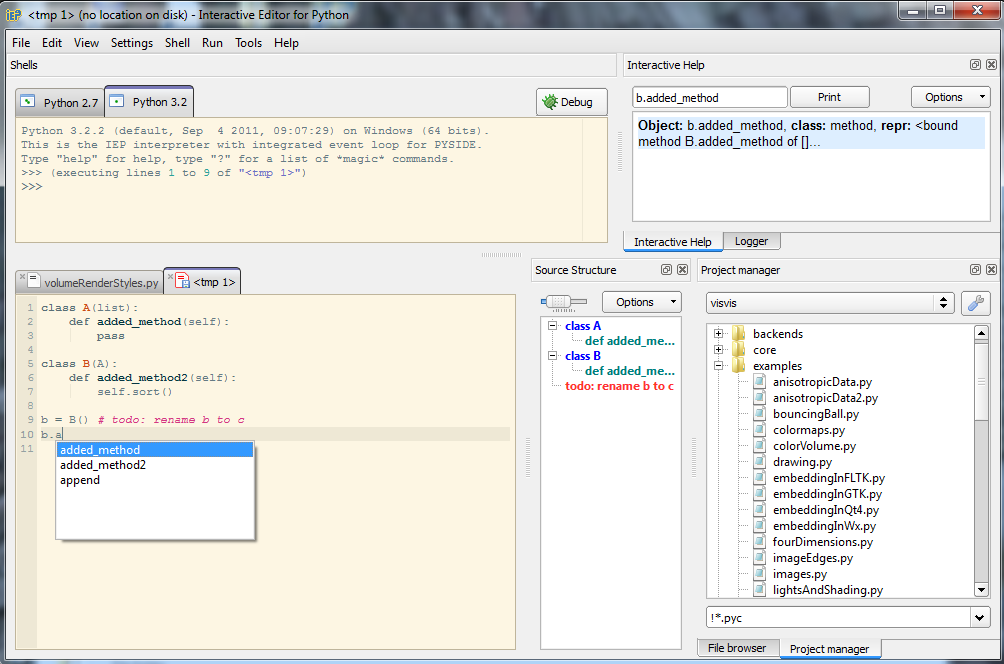
\includegraphics[height=0.5\textheight]{screen_pyzo.png}
		\caption{Pyzo.}
	\end{figure}
	
	
\end{frame}

\section{Calculs élémentaires}

\begin{frame}[fragile]
	\frametitle{Premiers pas}
	\begin{exo}
		On va commencer par se familiariser avec les opérations arithmétiques de base que peut faire Python.
		
		\begin{description}[<+->]
		\item[Addition] Entrer \lstinline|2+2| dans la console, appuyer sur \lstinline|Entrée| pour exécuter votre saisie. Vérifier que ça fait \lstinline|4|.
		\item[Soustraction] Entrer \lstinline|4-3|. Vérifier que l'on trouve \lstinline|1|.
		\item[Produit] Taper \lstinline|2*3|. Vérifier que l'on trouve \lstinline|6|.
		\item[Division] Taper \lstinline|12/3|. Vérifier que l'on trouve \lstinline|4|. Taper \lstinline|4/5|. Vérifier que l'on trouve \lstinline|0.8|.
		\item[...de CM1] Taper \lstinline|13//4|, et \lstinline|13%4|. Compléter la division posée suivante:
			\[
			\begin{array}{c|c}
			13      & 4\\ \cline{2-2}
			\ldots  & \ldots
			\end{array}
			 \]
			Que remarquez-vous ?
		\item[Puissances] Taper \lstinline|2**3|. Quel est le résultat ? Et celui de \lstinline|3**2| ?
		\end{description}
	\end{exo}
\end{frame}

\section{Variables}

\begin{frame}[fragile]
\frametitle{Variables}

Mais Python est bien plus puissant qu'une simple \textit{Casio collège}...
\pause

Une \textit{variable} est la donnée d'un emplacement mémoire où une valeur est stockée, et d'un nom.
\pause

Le fait d'affecter une valeur à une variable s'appelle une << \textit{affectation} >>. En Python, on fait ça avec une expression de la forme \lstinline|x=...|	
\pause

On peut également réaffecter une variable en recyclant simplement son nom.
\pause

Pour afficher la valeur d'une variable, on peut demander à Python de l'évaluer en tapant son nom.
\pause
	\begin{exo}
		
		\begin{itemize}[<+->]
		\item Créer une variable $x$ qui a la valeur $3$. Est-ce qu'on peut écrire \lstinline|3=x| ?
		
		\item Créer une variable $y$ qui a la valeur $7x$. Modifier la valeur de $x$. Cela modifie-t-il la valeur de $y$ ?
		
		\item Rajouter $1$ à $x$ en la réaffectant, vérifier en évaluant. Même question avec $0.5$.
		
		\item Que font \lstinline|x+=1|, \lstinline|x-=1|, \lstinline|x*=2| ou encore \lstinline|x/=2| ?
		
		\item Entrer l'instruction \lstinline|x,y=y,x|. Quelles sont alors les valeurs de $x$ et de $y$ ?
		\end{itemize}
		\pause[8]
	\end{exo}
\end{frame}

\begin{frame}[fragile]
	\textbf{Remarque} Dans un langage de programmation un peu plus \textit{kasher}, on déclare et on affecte séparément une variable. Mais Python permet de déclarer une variable directement par affectation.
	\pause
	
	\vspace{1em}
	\textbf{À propos des types}
	
	La fonction \lstinline|type|, appliquée à une variable $x$ via l'instruction \lstinline|type(x)|, renvoie le type de la variable $x$. Essayez sur plusieurs valeurs: \lstinline|type(0)|, \lstinline|type(0.5)|, \lstinline|type(type)|, et \lstinline|type(0.)|.
	\pause
	
	Les types \lstinline|int| et \lstinline|float| servent respectivement à représenter les nombres entiers et les nombres réels à virgule dans Python. On peut faire les opérations arithmétiques vues plus haut avec elles, même quand les variables en jeu sont d'un type et de l'autre.
	
\end{frame}

\section{Chaînes de caractères}
\subsection{Généralités}

\begin{frame}[fragile]{Chaînes de caractères}{Généralités}
Un nouveau type de variable important: le type \lstinline|str|, pour \textit{string} ou \textit{chaîne de caractères}, en français. On peut les définir explicitement en incluant son message entre guillemets simples (\lstinline|'|) ou doubles (\lstinline|"|).\pause

Il faut faire attention : quand on démarre par une guillemet d'un type, l'apparition d'une autre guillemet du même type clôt la chaîne.\pause

	\begin{exo}
	
	\begin{itemize}[<+->]
	\item Définir une variable \lstinline|Bonjour| prenant la valeur $0$.
	
	\item Que fait \lstinline|print(Bonjour)| ? Et les instructions \lstinline|print("Bonjour")| et \lstinline|print('Bonjour')| ?
	
	\item Comparer \lstinline|type(Bonjour)|, \lstinline|type('Bonjour')| et \lstinline|type("Bonjour")|.
	
	\item Évaluer \lstinline|len("Bonjour")|. À quoi cela correspond-t-il ?
    
    \item Afficher \lstinline|J'aime la tartiflette| et  \lstinline|Il dit: "Bonjour !"|. Attention à utiliser des types de guillemets différents !
    \end{itemize}
\end{exo}

\end{frame}

\subsection{Opérations sur les chaînes}

\begin{frame}[fragile]{Chaînes de caractères}{Opérations}


	\begin{exo}
    \begin{itemize}[<+->]
	
	
	\item Que se passe-t-il quand on affiche une chaîne contenant \lstinline|\n| ?
	
	\item Définir deux chaines de caractères \lstinline|x| et \lstinline|y|: que fait \lstinline|print(x, y)| ? Est-ce que ça marche aussi si \lstinline|x| est une variable de type \lstinline|int| ?
	
	\item Évaluer la valeur de \lstinline|x+y|, l'afficher via \lstinline|print|.
	
	\item Afficher << \lstinline|1/100 est petit| >> en remplaçant \lstinline|1/100| par sa valeur. On utilisera \lstinline|"{} est petit".format()| où \lstinline|x| est la valeur voulue.
	
	\end{itemize}
	\end{exo}
\end{frame}

\section{Premiers programmes}

\begin{frame}[fragile]
	\frametitle{Premiers programmes}
	
	On va maintenant basculer sur la zone d'écriture de scripts. Un programme est une succession d'instructions qui sont effectuées lorsqu'il est exécuté.
	\pause
	
	\begin{exo}
	\begin{itemize}[<+->]
	\item Écrire un programme qui stocke la chaîne << \lstinline|Bonjour| >> dans une variable \lstinline|x|, puis l'affiche, puis affiche << \lstinline|Bonjour Bonjour| >>.
	
	\item Écrire un programme qui demande à l'utilisateur d'entrer un texte, affiche << \lstinline|Vous avez entré:| >> suivi du texte entré. On utilisera la fonction \lstinline|input|:	
	\begin{lstlisting}
	texte = input()
	\end{lstlisting}
	demande, à son exécution, une chaîne de caractère à l'utilisateur, puis la stocke dans la variable \lstinline|texte|.
	
	\item Écrire un programme qui demande à l'utilisateur un nombre, le stocke dans une variable \lstinline|x|, puis affiche << \lstinline|f(x) = | >> suivi de la valeur de $\frac{1}{1+x^2}$. On pourra utiliser \lstinline|input|, convertir son entrée (initialement de type \lstinline|str|) en un entier via le constructeur \lstinline|int|.
	
	\end{itemize}
	\end{exo}
\end{frame}


\end{document}